%==========================================================================
\chapter{Structured-Grid Interface}
\label{Structured-Grid Interface}

In order to get access to the most efficient and scalable solvers for
structured-grid applications, users should use the \code{Struct}
interface described in this chapter.  This interface will also provide
access (this is not yet supported) to solvers in \hypre{} that were
designed for unstructured-grid applications and sparse linear systems
in general.  These additional solvers are usually provided via the
unstructured-grid interface (\code{FEI}) or the linear-algebraic
interface (\code{IJ}) described in Chapters \ref{chapter-FEI} and
\ref{chapter-IJ}.

Figure \ref{fig-fv-grid} gives an example of the type of grid
currently supported by the \code{Struct} interface.
\begin{figure}
\centering
\includegraphics[width=4in]{fv_grid.eps}
\caption{%
An example 2D finite-volume grid, distributed accross two processors.}
\label{fig-fv-grid}
\end{figure}
The interface uses a finite-difference or finite-volume style, and
currently supports only scalar PDEs (i.e., one unknown per gridpoint).
There is an effort to extend it to use a finite-element style (similar
to the \code{FEI}, but on structured grids), and to support PDE systems.

There are four basic steps involved in setting up the linear system
to be solved:
\begin{itemize}
\item set up the grid,
\item set up the stencil,
\item set up the matrix,
\item set up the right-hand-side.
\end{itemize}
To describe each of these steps in more detail, consider solving the
2D Laplacian problem
\begin{equation}\label{eqn-laplacian}
\left \{
\begin{array}{ll}
\nabla^2 u = f , & \mbox{in the domain}, \\
u = 0,           & \mbox{on the boundary}.
\end{array}
\right .
\end{equation}
Consider discretizing (\ref{eqn-laplacian}) using standard 5-pt
finite-volumes on the uniform grid in \ref{fig-fv-grid}.

%==========================================================================

\section{Setting Up the Grid}
\label{Setting Up the Grid}

%==========================================================================

\section{Setting Up the Stencil}
\label{Setting Up the Stencil}

%==========================================================================

\section{Setting Up the Matrix}
\label{Setting Up the Matrix}

%==========================================================================

\section{Setting Up the Right-Hand-Side}
\label{Setting Up the Right-Hand-Side}

%==========================================================================




Now test the \code{display} environment.
\begin{display}
\begin{verbatim}
HelloThere;
i = 9;
\end{verbatim}
\end{display}
Now add another sentence.
